\begin{figure*}
	\begin{center}
		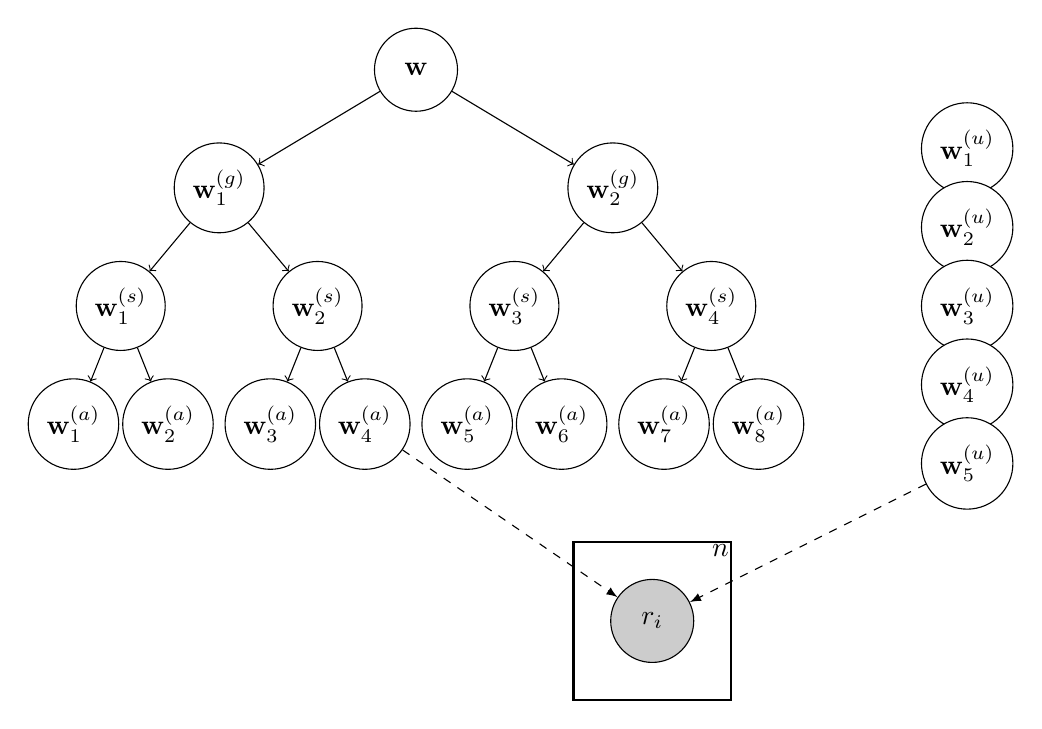
\begin{tikzpicture}[darkstyle/.style={circle,draw,fill=white!40,minimum size=30}]
		\tikzstyle{obsnode}=[circle,draw,fill=gray!40,minimum size=30]
		\tikzstyle{plate}=[draw,thick,minimum width=2cm,minimum height=2cm]
		\tikzstyle{line}=[draw]
		\tikzstyle{arrow}=[draw, -latex,dashed]
		\tikzstyle{level 1}=[sibling distance=50mm]
		\tikzstyle{level 2}=[sibling distance=25mm]
		\tikzstyle{level 3}=[sibling distance=12mm]
		\tikzstyle{level 4}=[sibling distance=6mm]
		\tikzstyle{level 5}=[sibling distance=4mm,level distance=10mm]
		\node[darkstyle]{\textbf{w}} child[->] foreach \g in {1,2}
		{node[darkstyle] {$\textbf{w}^{(g)}_{\g}$} child[->] foreach \t [evaluate={\s=int(\g*2+\t-1);}] in {0,1}
			{ node[darkstyle] {$\textbf{w}^{(s)}_{\s}$} child[->] foreach \q [evaluate={\a=int(\s*2+\q-1);}] in {0,1}
				{node[darkstyle] (a\a) {$\textbf{w}^{(a)}_{\a}$} }}};
		\foreach \u in {1,...,5}
		{\pgfmathtruncatemacro{\label}{\u}
			\node[darkstyle] (u\u) at (7,0-\u){$\textbf{w}^{(u)}_\label$};}
		
		\node[plate] (p) at (3,-7){} ;
		\node[obsnode](r) at (3,-7){$r_{i}$};
		\node[anchor=north east,inner sep=1pt] at (p.north east){$n$};
		\path[arrow]  (u5) -- (r){};
		\path[arrow]  (a4) -- (r){};
		
		\end{tikzpicture}
	\end{center}
	\caption{A Graphical Representation of the Model}
	\label{fig:graphical_model}
\end{figure*}